\section{Musical Preliminaries}
\label{sec:music}

\paragraph{Pitches}
In music, a \emph{pitch} is a value denoting how high or low a sound is.
Pitches can be represented either as an absolute value or as a relative
value paired with the octave the sound belongs to.
In our implementation, the two representations of pitches are defined
as \texttt{Pitch} and \texttt{PitchOctave}, respectively, accompagnied
by a proof that converting back and forth between them is an identity.

\begin{alltt}
data Pitch : Set where
  pitch : \(\mathbb{N}\) \(\rightarrow\) Pitch

data Octave : Set where
  octave : \(\mathbb{N}\) \(\rightarrow\) Octave

PitchOctave : Set
PitchOctave = Fin 12 \(\times\) Octave
\end{alltt}

\paragraph{Duration}
\emph{Duration} denotes a certain unit of time during which a sound
or silence lasts.
The unit is unspecified at the composition time; it is instantiated to
a concrete value when the music is played at a specific tempo.

\begin{alltt}
data Duration : Set where
  duration : \(\mathbb{N}\) \(\rightarrow\) Duration
\end{alltt}

\paragraph{Note}
Combining pitches and duration gives us \emph{notes}.
In our implementation, we represent notes with sound as \texttt{tone}s
and those without as \texttt{rest}s.

\begin{alltt}
data Note : Set where
  tone : Duration \(\rightarrow\) Pitch \(\rightarrow\) Note
  rest : Duration         \(\rightarrow\) Note
\end{alltt}

\paragraph{Intervals}

\emph{Intervals} are yet another key concept in music.
An interval denotes the difference in pitch between two notes.
There are 13 kinds of interval within an octave, and these intervals
may be classified from several different perspectives: (i) major or minor;
(ii) consonant or dissonant; and (iii) perfect or imperfect.
For convenience, we let the names of intervals carry the information
about the first and third classifications.
As a convention, we refer to \texttt{min2} and \texttt{maj2}  uniformly
as ``2nd'', and similarly for other intervals.
We also call \texttt{per1} the \emph{unison} in the rest of this section.

\begin{figure}[h]
  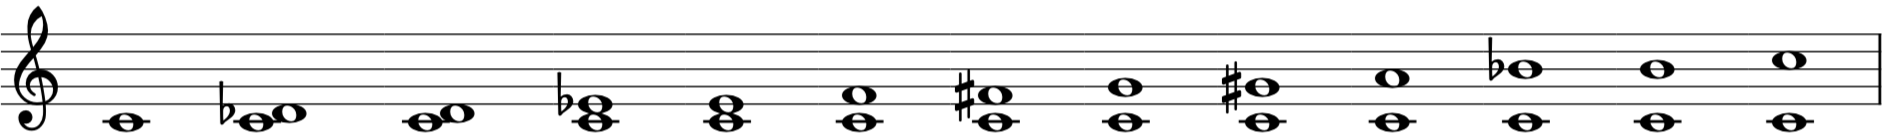
\includegraphics[width=12cm]{interval.png} \\
  \begin{flushleft}
    \begin{small}
      \hspace{1.45cm} per1 \ \ \ min2 \ \ \ \ maj2 \ \ \ min3 \ \ maj3
      \ \ per4 \ \ aug4 \ \ \,per5 \ \ min6 \ \,maj6 \ \,min7 \ \,maj7 \ \,per8
    \end{small}
  \end{flushleft}
\end{figure}
  
\begin{alltt}
data Interval : Set where
interval : \(\mathbb{N}\) \(\rightarrow\) Interval

per1  = interval 0 -- consonant
min2  = interval 1
maj2  = interval 2
min3  = interval 3 -- consonant
maj3  = interval 4 -- consonant
per4  = interval 5 
aug4  = interval 6
per5  = interval 7 -- consonant
min6  = interval 8 -- consonant
maj6  = interval 9 -- consonant
min7  = interval 10
maj7  = interval 11
per8  = interval 12 -- consonant
\end{alltt}
